\documentclass{article}
\usepackage{v-equation}
\vgeometry

\begin{document}

\def\gdrive{https://drive.google.com/drive/folders/13jDlDu3dqgqlrGpexnhM-_973XcsRNFk?usp=share_link}
\vtitle[Radius : Circular path in a uniform magnetic field]
\begin{center}
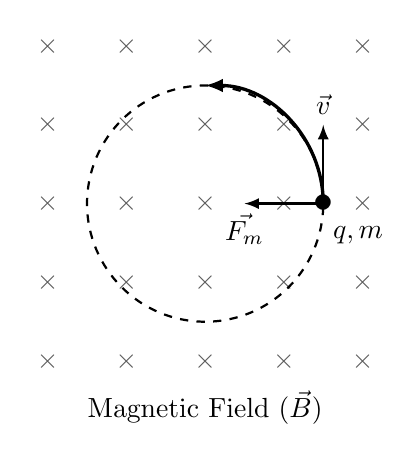
\begin{tikzpicture}
[xscale=1, yscale=1, >=latex]
\foreach \x in {-2,...,2} \foreach \y in {-2,...,2} { \node at (\x, \y)[opacity=0.65]{$\times$};}
\draw[thick,dashed] (0,0) circle[radius=1.5];
\node at (1.5,0)[below=4 mm, right]{$q, m$};
\draw[->, thick] (1.5,0)--(1.5,1)node[above]{$\vec{v}$};
\draw[->, thick] (1.5,0)--(0.5,0)node[below]{$\vec{F_m}$};
\draw[->, very thick] (1.5,0) arc[start angle=0, end angle=90, radius=1.5];
\node at (0,-2.25)[below]{Magnetic Field ($\vec{B}$)};
\node at (1.5,0) {\Large{$\bullet$}};
\end{tikzpicture}
\end{center}
\vspace*{\fill}
\begin{align*}
\vec{F}_{\textit{magnetic}} & =\vec{F}_{\textit{centripetal}}\\
qvB & = \dfrac{mv^2}{r} \\
r & = \dfrac{mv^2}{qvB}\\
r & = \dfrac{mv}{qB}
\end{align*}
\vspace*{\fill}

\pagebreak

\vspace*{\fill}
\begin{center}
    \fbox{\qrcode[height=2cm]{\gdrive}}
\end{center}
\vspace*{\fill}
\end{document}
